\chapter{Probability Distributions}

\section{Introduction}

In this lab, you will create your own simulation of a binomial
process, and compare the results of your simulation with the PDFs for
the binomial, Poisson, and Gaussian processes in the appropriate
limits.

This lab includes a number of code snippets to illustrate the ideas
that are being discussed.  However, the entire source listing is not
available to you, as this would amount to giving away the answer.  You
will also notice that most of the code snippets cannot be cut and
pasted.  This is all intentional.  The examples should help you
understand what you should do, but you will have to write your own
code.  {\bf Do not expect the code snippets as written to work for
your code without any modification... they are not supposed to!}

\section{Simulating the Binomial Process}

Your first task is to create a Monte Carlo simulation for a binomial
process.  The Monte Carlo method, named after the casino in Monaco, refers
to the repeated sampling of random variables to obtain numerical results.

Suppose one single experiment consists of $n_{\rm try}$ trials with a
probability $\epsilon$ of success.  The outcome of each experiment is
a single number from 0 to $n_{\rm try}$ reporting the number of the
$n_{\rm try}$ trials from that particular experiment which were
successful.  To study the distribution of outcomes, you will repeat the
experiment $n_{\rm exp}$ times.

There are libraries functions that will simulate this process for you,
but for this lab you will create your own simulation.  While
developing your code, start with a small test. For instance $n_{\rm
  try} = 3$ and $n_{\rm exp}=5$, as shown in the example below.
Implement your Monte Carlo simulation in the following manner:
\begin{itemize}
\item Create a 2-D array of shape $n_{\rm exp}$ by $n_{\rm try}$
  filled with random values chosen uniformly from 0 to 1.0:\\
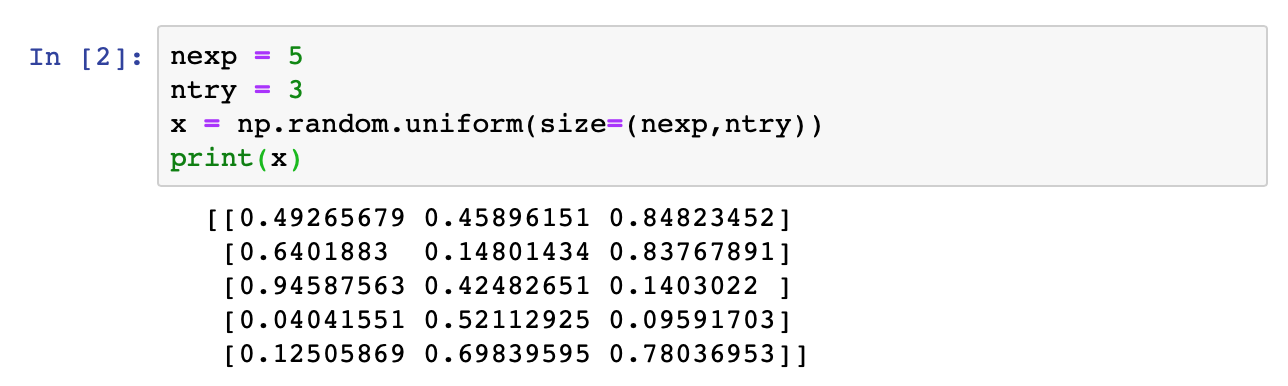
\includegraphics[width=0.85\textwidth]{figs/labs/distributions/makearray.png} \\
This array associates a random value with each trial from each
experiment.  
\item Consider a trial successful if the randomly chosen value is less
  than $\epsilon$.  In this example, taking $\epsilon = 0.5$ and
  assuming 1 indicates success and 0 a failure, we obtain:
\begin{samepage}
\begin{verbatim}
[[1 1 0]
 [0 1 0]
 [0 1 1]
 [1 0 1]
 [1 0 0]]
\end{verbatim}
\end{samepage}
In the first simulated experiment, the first two trials were
successful and the last trial failed.  In the second experiment, the
first trial failed, the next trial was successful, and the last trial
failed.  And so on.

\item Next, count the number of trials that were successful in each experiment.  The result will be a 1-D array of length $n_{\rm exp}$.  Consider using the {\tt np.sum} function with the {\tt axis} parameter.  In this example, we obtain the array of outcomes $m$:
\begin{verbatim} 
[2 1 2 2 1]
\end{verbatim}
This is the outcome of our five simulated experiments.  The first
experiment has two out of three trials successful, the second
experiment had one out of three trials successful, and so on.
\end{itemize} 
Work through the example and make sure you see how each result follows
from the previous step.  Then implement and test your own version in
Scientific Python.  When validating a numerical calculation, think hard
about good test cases.  For instance, if you only test with the value
of $\epsilon = 0.5$, you won't catch a bug that mistakes success for
failure.  Try a few different test cases, with reasonably small values
for $n_{\rm try}$ and $n_{\rm exp}$ and check your numerical
simulation.  Boundaries often make a good check, for instance
$\epsilon = 0$ and $\epsilon = 1$.

Another effective validation strategy is to check known mathematical
relations using your simulation.  For instance, we know that the mean
value of a Binomial distribution is given by:
\begin{equation} \label{eqn:binom_mean}
\bar{m} = n_{\rm try} \cdot \epsilon
\end{equation}
and that the variance is given by:
\begin{equation} \label{eqn:binom_var}
\sigma^2 = n_{\rm try} \cdot \epsilon \, (1 - \epsilon)
\end{equation}
and so these predicted values, calculated from your parameters
$\epsilon$ and $n_{\rm try}$ can be compared to the mean and variance
of the outcome array $m$ from your simulation, calculated using the numpy functions {\tt np.mean} and {\tt np.var}.  A
comparison with $n_{\rm exp}=1000$, $n_{\rm try}=10$, and
$\epsilon=0.5$ should result in something like:\\
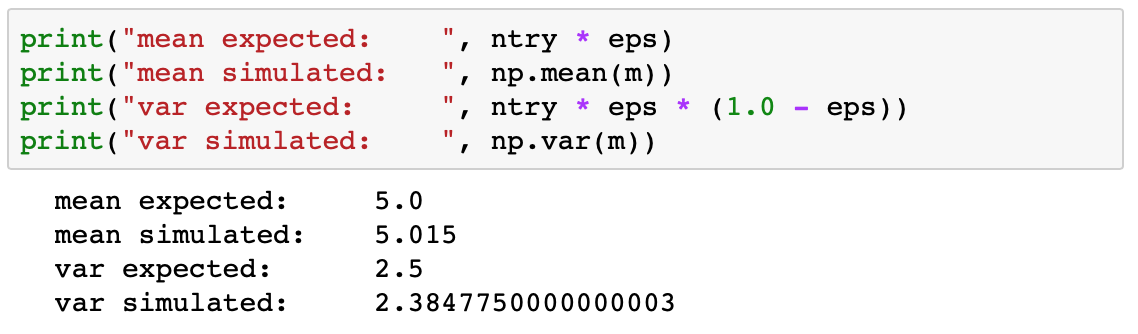
\includegraphics[width=0.85\textwidth]{figs/labs/distributions/validate.png}\\ 
Produce a large number of pseudo-experiments by setting $n_{\rm exp} =
1000$ and comment out any debugging print statements which will get
very long.  Pick five well chosen test cases with different values of
$n_{\rm try}$ and $\epsilon$ and compare the expected and simulated
mean and variances.  The simulated values will fluctuate by a
fractional amount $1/\sqrt{n_{\rm exp}}$.  So for $n_{\rm exp} =
1000$, we expect the expected and simulated values to agree within
about $3\%$.  If you increase to $n_{\rm exp} = 100000$, the agreement
should improve to better than $1\%$.  Be certain to record your test
cases and the results in your logbook.

\section{Histogram for the Binomial Process}

We use histograms to represent the distribution of numerical data.
Fill an output array $m$ with the results of $n_{\rm exp} = 1000$
experiments each consisting of $n_{\rm try}=10$ trials with success rate
$\epsilon=0.25$.  There are eleven possible outcomes for each of these
experiments: $0,1,2,\ldots,10$.  Construct a histogram from these 1000
outcomes using the {\tt np.histogram} function:\\
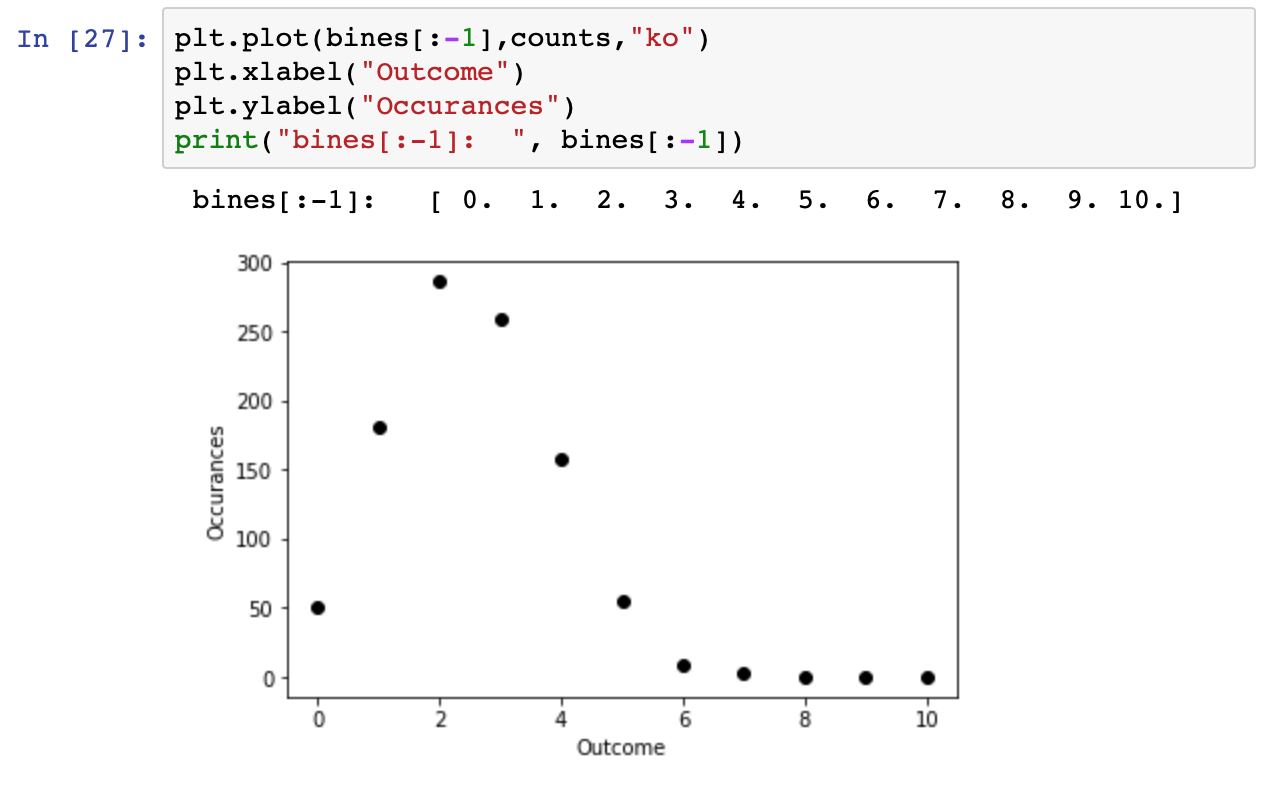
\includegraphics[width=0.85\textwidth]{figs/labs/distributions/makehist.png} \\
This calculates a histogram with eleven bins covering the range from
zero to eleven, and reports the number of outcomes from $m$ that occur
in each bin.  It returns two arrays, which we save as {\tt counts} and
{\tt bines}.  We interpret the outcome of the {\tt counts} array as follows:  60
experiments have zero successes, 164 experiments have one success, 281
experiments have two successes, and so on.  The exact values will vary
each time you run the simulation, but in all cases the sum across all
bins should equal the total number of experiments $n_{\rm exp} =
1000$.

Histograms are designed to handle continuous data, so you have to take a bit of care when using them to display discrete data (integers) as we are doing here.  Consider the bin edges array {\tt bines} that was returned in this example:
\begin{verbatim}
   bin edges:   [ 0.  1.  2.  3.  4.  5.  6.  7.  8.  9. 10. 11.]
\end{verbatim}
which you will notice has length 12.  This is because the
array contains the {\bf edges} of eleven consecutive bins.  Technically the first bin
is the count of all outcomes in the range from zero (inclusive) to
just below one (exclusive).  The next bin is the count of all outcomes
in the range from one (inclusive) to just below two (exclusive).  In
this case, however, we are using discrete data, and so there are no entries with values like 1.73 to consider.
All the entries in the first bin are from experiments with the outcome
zero, while all the entries in the second bin are from the outcome
one.  The best way to plot this histogram from discrete data, therefore, is
to associate each count with the leading bin edge, that is:\\
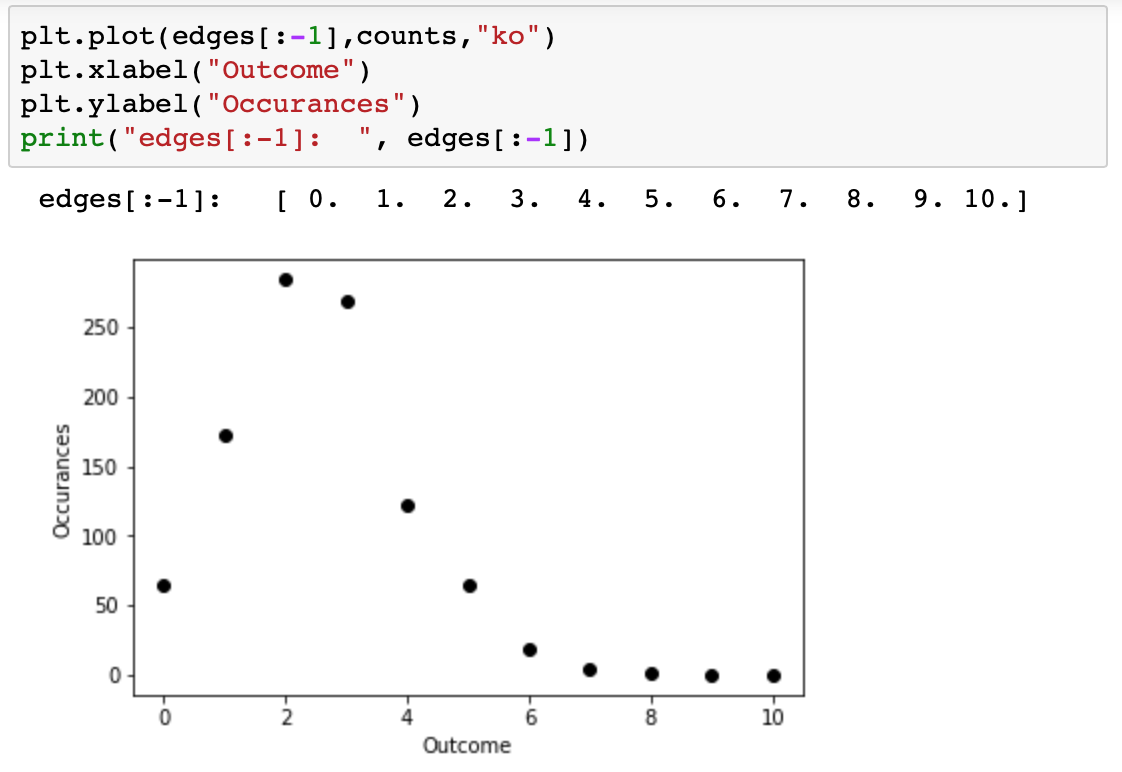
\includegraphics[width=0.85\textwidth]{figs/labs/distributions/plothist.png} \\
Notice the essential trick for plotting {\em discrete} data is to use the slice {\tt bines[:-1]} of the bin edges data
\begin{verbatim}
   bines[:-1]:   [ 0.  1.  2.  3.  4.  5.  6.  7.  8.  9. 10.]
\end{verbatim}
as the $x$ values for plotting the occurances of each outcome.  This
slice (all but the last entry) essentially throws out the superfluous
bin edge 11.  (This trick only works for discrete data!)  Notice that
in our final plot, we have the number of occurances at each of the
eleven possible outcomes correctly centered over the numbers
$0,1,2,\ldots,10.$


\pagebreak

\section{Comparison with Binomial PDF}

Next we'd like to compare our Monte Carlo simulation with the PDF for
the binomial distribution.  We'll use the {\tt scipy.stats.binom.pmf}
function, which is the PDF for the discrete binomial distribution
available in Scientific Python.  This PDF is only non-zero at integer
values, so we'll simply evaluate it at each discrete occurance,
i.e. the same slice {\tt bines[0:-1]} which we used to plot the
histogram:\\
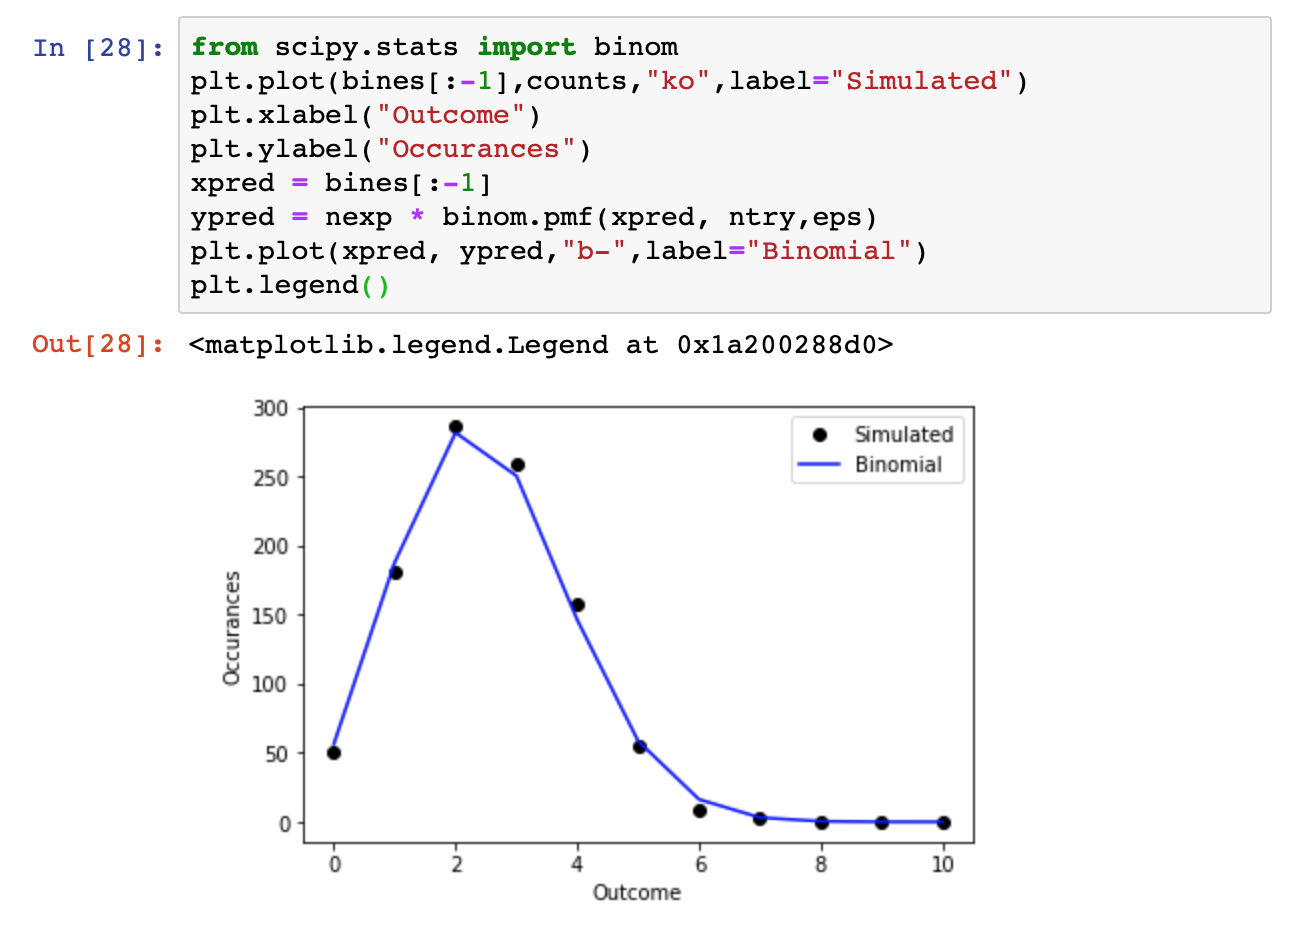
\includegraphics[width=0.85\textwidth]{figs/labs/distributions/compare.png}
\\ Notice that we scale the PDF by the number of experiments $n_{\rm
  exp}$.  The PDF is the expected frequency of each outcome for a
single experiment, but we are plotting the number of occurrences for
$n_{\rm exp}$ experiments.

{\bf Plots 1-3:}  Compare the output of your Monte Carlo simulation with the Binomial
distribution PDF with $n_{\rm exp} = 1000$ and $n_{\rm try} = 20$, and
for three different values of $\epsilon$: 0.25, 0.5, and 0.75.  


\section{The Poisson Limit}

The Poisson distribution follows from the Binomial distribution in the
limit that $n_{\rm try} \to \infty$.  Recall that the mean value of
the Poisson distribution is $\bar{m} = \epsilon \, n_{\rm try}$.  If
we kept the success rate $\epsilon$ as a parameter, than any finite
value of $\epsilon$ would cause the mean of the distribution to diverge to infinity.
If instead we hold the mean value to the constant value $\lambda$, by taking:
\begin{displaymath}
\epsilon = \frac{\lambda}{n_{\rm try}}
\end{displaymath}
we see that $\epsilon \to 0$ as $n_{\rm try} \to \infty$ and the mean
of the Poisson distribution remains at the fixed value $\lambda$.

We'll explore this limit numerically simply by taking $n_{\rm try}$ to
the large (but finite) value of 10,000.  To produce a Poisson distribution with $\lambda = 2$, set the parameters of the binomial simulation like:
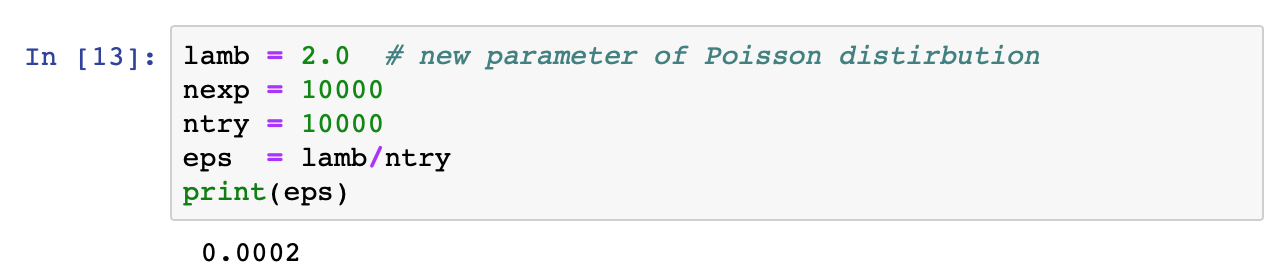
\includegraphics[width=0.85\textwidth]{figs/labs/distributions/poissonlimit.png}\\
After setting the parameters in this way, rerun your Monte Carlo simulation of the binomial process and save the array of outcomes $k$.  Plot the outcome as a histogram as before, but instead of comparing to the Binomial distribution PDF, compare to the Poisson distribution PDF with $\lambda = 5$:\\
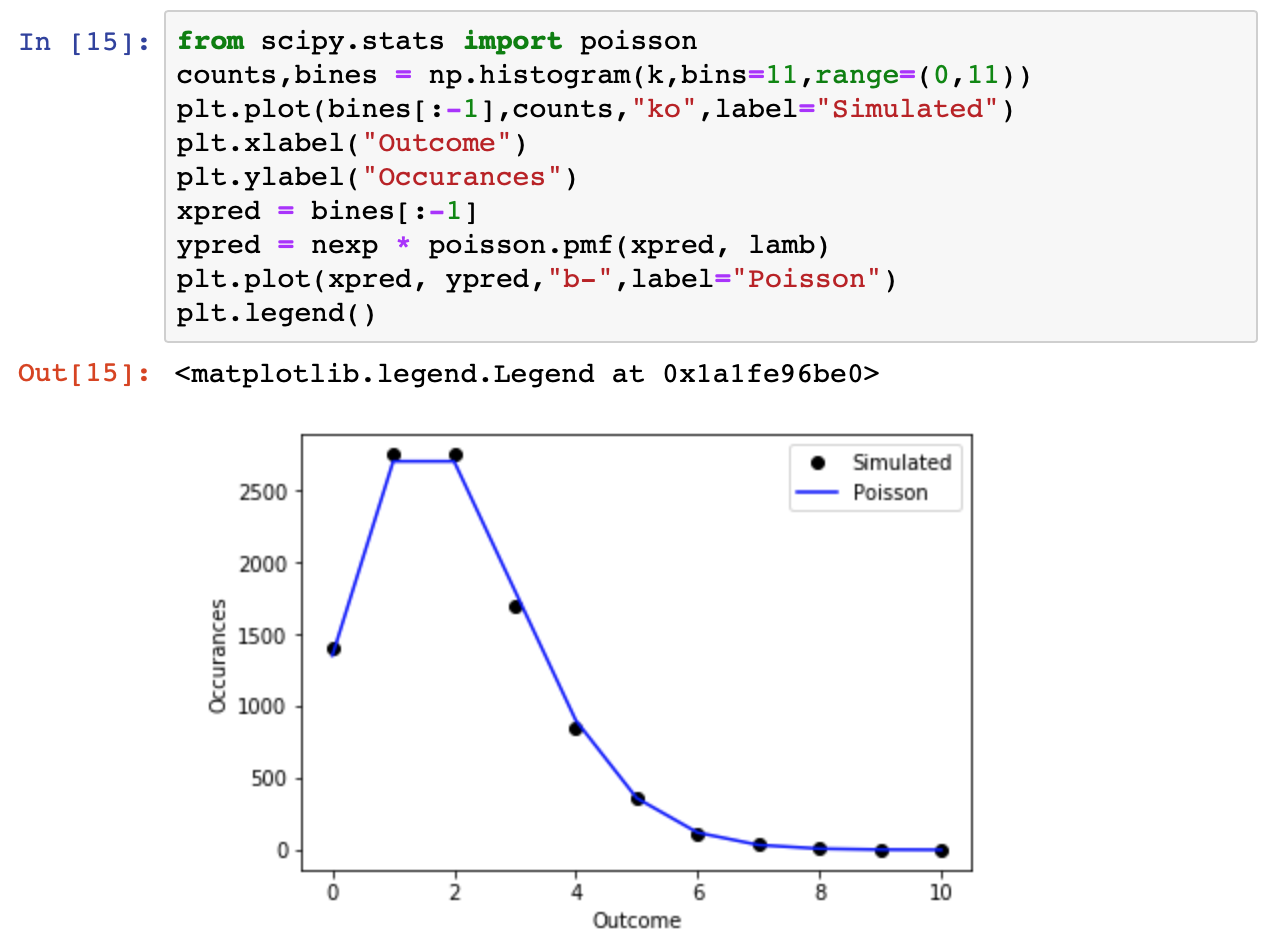
\includegraphics[width=0.85\textwidth]{figs/labs/distributions/poisson.png}\\

{\bf Plots 4-5:}  In the Poisson limit, compare the output of your Monte Carlo simulation to the Poisson PDF
for two different values of $\lambda$:  3.0, 5.2.  Use eleven bins: 0,1,2,...,10.

Using {\tt np.mean} and {\tt np.var}, check that mean and variance of
your distributions is as you expect in each case, and record the
results in your log book.

\section{The Gaussian Limit}

As the mean value $\lambda$ of the Poisson distribution gets larger, the Poisson distribution resembles the Gaussian distribution.  You can plot the PDF of the Gaussian distribution using the {\tt scipy.stats.norm.pdf} function:\\
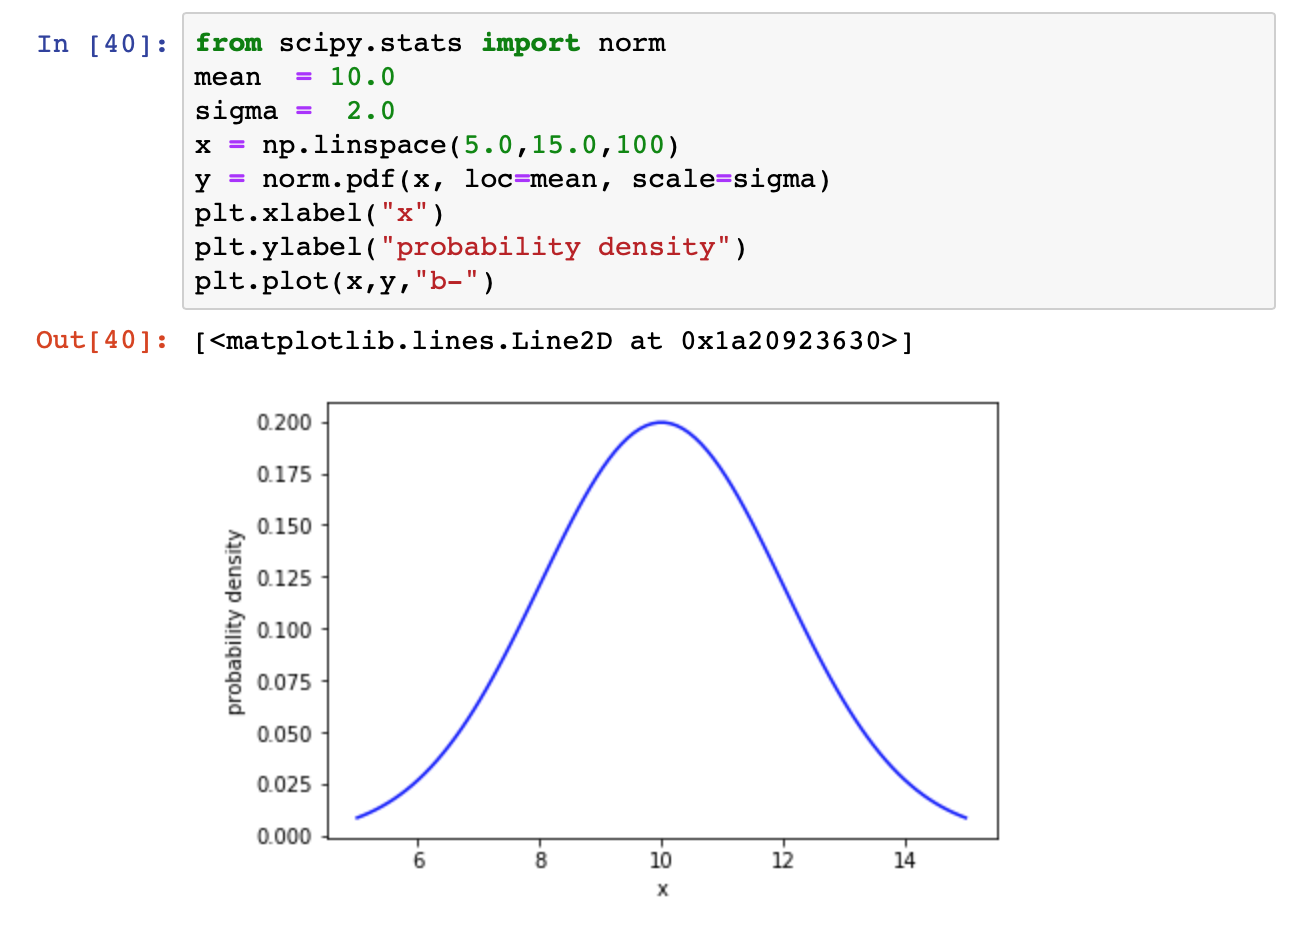
\includegraphics[width=0.85\textwidth]{figs/labs/distributions/plotgauss.png}\\
The parameter names are a bit strange for this scipy function.  Set the parameter {\tt loc} to the mean value, and the parameter {\tt scale} to $\sigma$.  Recall that in the Poisson limit $\sigma^2 = \lambda$.

{\bf Plots 6:} Compare the output your Monte Carlo simulation to the Gaussian PDF for $\lambda = 100$.  Use 60 bins:  70,71,72,...,130

















